% Options for packages loaded elsewhere
% Options for packages loaded elsewhere
\PassOptionsToPackage{unicode}{hyperref}
\PassOptionsToPackage{hyphens}{url}
\PassOptionsToPackage{dvipsnames,svgnames,x11names}{xcolor}
%
\documentclass[
  letterpaper,
  DIV=11,
  numbers=noendperiod]{scrartcl}
\usepackage{xcolor}
\usepackage{amsmath,amssymb}
\setcounter{secnumdepth}{5}
\usepackage{iftex}
\ifPDFTeX
  \usepackage[T1]{fontenc}
  \usepackage[utf8]{inputenc}
  \usepackage{textcomp} % provide euro and other symbols
\else % if luatex or xetex
  \usepackage{unicode-math} % this also loads fontspec
  \defaultfontfeatures{Scale=MatchLowercase}
  \defaultfontfeatures[\rmfamily]{Ligatures=TeX,Scale=1}
\fi
\usepackage{lmodern}
\ifPDFTeX\else
  % xetex/luatex font selection
\fi
% Use upquote if available, for straight quotes in verbatim environments
\IfFileExists{upquote.sty}{\usepackage{upquote}}{}
\IfFileExists{microtype.sty}{% use microtype if available
  \usepackage[]{microtype}
  \UseMicrotypeSet[protrusion]{basicmath} % disable protrusion for tt fonts
}{}
\makeatletter
\@ifundefined{KOMAClassName}{% if non-KOMA class
  \IfFileExists{parskip.sty}{%
    \usepackage{parskip}
  }{% else
    \setlength{\parindent}{0pt}
    \setlength{\parskip}{6pt plus 2pt minus 1pt}}
}{% if KOMA class
  \KOMAoptions{parskip=half}}
\makeatother
% Make \paragraph and \subparagraph free-standing
\makeatletter
\ifx\paragraph\undefined\else
  \let\oldparagraph\paragraph
  \renewcommand{\paragraph}{
    \@ifstar
      \xxxParagraphStar
      \xxxParagraphNoStar
  }
  \newcommand{\xxxParagraphStar}[1]{\oldparagraph*{#1}\mbox{}}
  \newcommand{\xxxParagraphNoStar}[1]{\oldparagraph{#1}\mbox{}}
\fi
\ifx\subparagraph\undefined\else
  \let\oldsubparagraph\subparagraph
  \renewcommand{\subparagraph}{
    \@ifstar
      \xxxSubParagraphStar
      \xxxSubParagraphNoStar
  }
  \newcommand{\xxxSubParagraphStar}[1]{\oldsubparagraph*{#1}\mbox{}}
  \newcommand{\xxxSubParagraphNoStar}[1]{\oldsubparagraph{#1}\mbox{}}
\fi
\makeatother


\usepackage{longtable,booktabs,array}
\usepackage{calc} % for calculating minipage widths
% Correct order of tables after \paragraph or \subparagraph
\usepackage{etoolbox}
\makeatletter
\patchcmd\longtable{\par}{\if@noskipsec\mbox{}\fi\par}{}{}
\makeatother
% Allow footnotes in longtable head/foot
\IfFileExists{footnotehyper.sty}{\usepackage{footnotehyper}}{\usepackage{footnote}}
\makesavenoteenv{longtable}
\usepackage{graphicx}
\makeatletter
\newsavebox\pandoc@box
\newcommand*\pandocbounded[1]{% scales image to fit in text height/width
  \sbox\pandoc@box{#1}%
  \Gscale@div\@tempa{\textheight}{\dimexpr\ht\pandoc@box+\dp\pandoc@box\relax}%
  \Gscale@div\@tempb{\linewidth}{\wd\pandoc@box}%
  \ifdim\@tempb\p@<\@tempa\p@\let\@tempa\@tempb\fi% select the smaller of both
  \ifdim\@tempa\p@<\p@\scalebox{\@tempa}{\usebox\pandoc@box}%
  \else\usebox{\pandoc@box}%
  \fi%
}
% Set default figure placement to htbp
\def\fps@figure{htbp}
\makeatother





\setlength{\emergencystretch}{3em} % prevent overfull lines

\providecommand{\tightlist}{%
  \setlength{\itemsep}{0pt}\setlength{\parskip}{0pt}}



 


\usepackage{booktabs}
\usepackage{longtable}
\usepackage{array}
\usepackage{multirow}
\usepackage{wrapfig}
\usepackage{float}
\usepackage{colortbl}
\usepackage{pdflscape}
\usepackage{tabu}
\usepackage{threeparttable}
\usepackage{threeparttablex}
\usepackage[normalem]{ulem}
\usepackage{makecell}
\usepackage{xcolor}
\usepackage{fvextra}
\DefineVerbatimEnvironment{Highlighting}{Verbatim}{breaklines,commandchars=\\\{\}}
\KOMAoption{captions}{tableheading}
\makeatletter
\@ifpackageloaded{caption}{}{\usepackage{caption}}
\AtBeginDocument{%
\ifdefined\contentsname
  \renewcommand*\contentsname{Table of contents}
\else
  \newcommand\contentsname{Table of contents}
\fi
\ifdefined\listfigurename
  \renewcommand*\listfigurename{List of Figures}
\else
  \newcommand\listfigurename{List of Figures}
\fi
\ifdefined\listtablename
  \renewcommand*\listtablename{List of Tables}
\else
  \newcommand\listtablename{List of Tables}
\fi
\ifdefined\figurename
  \renewcommand*\figurename{Figure}
\else
  \newcommand\figurename{Figure}
\fi
\ifdefined\tablename
  \renewcommand*\tablename{Table}
\else
  \newcommand\tablename{Table}
\fi
}
\@ifpackageloaded{float}{}{\usepackage{float}}
\floatstyle{ruled}
\@ifundefined{c@chapter}{\newfloat{codelisting}{h}{lop}}{\newfloat{codelisting}{h}{lop}[chapter]}
\floatname{codelisting}{Listing}
\newcommand*\listoflistings{\listof{codelisting}{List of Listings}}
\makeatother
\makeatletter
\makeatother
\makeatletter
\@ifpackageloaded{caption}{}{\usepackage{caption}}
\@ifpackageloaded{subcaption}{}{\usepackage{subcaption}}
\makeatother
\usepackage{bookmark}
\IfFileExists{xurl.sty}{\usepackage{xurl}}{} % add URL line breaks if available
\urlstyle{same}
\hypersetup{
  pdftitle={Curiosity Project: Student Pilot Data Analysis (22-Oct-25)},
  colorlinks=true,
  linkcolor={blue},
  filecolor={Maroon},
  citecolor={Blue},
  urlcolor={Blue},
  pdfcreator={LaTeX via pandoc}}


\title{Curiosity Project: Student Pilot Data Analysis (22-Oct-25)}
\author{}
\date{}
\begin{document}
\maketitle

\RecustomVerbatimEnvironment{verbatim}{Verbatim}{
showspaces = false,
showtabs = false,
breaksymbolleft={},
breaklines
}

\renewcommand*\contentsname{Table of contents}
{
\hypersetup{linkcolor=}
\setcounter{tocdepth}{3}
\tableofcontents
}

The raw data from the student pilot test contained 267 responses. After
removing those who did not consent to participate, Aidan's test
responses, and respondents who do not reside in the U.S., the final
sample size is 263 respondents.

\section{Experimental Conditions}\label{experimental-conditions}

The random assignment to conditions appears to have worked fine. The
number of respondents per condition ranged from 56-63
(Table~\ref{tbl-aexpcond} and Table~\ref{tbl-rexpcond}).

\begin{table}

\caption{\label{tbl-aexpcond}Number of respondents in the control and
experimental conditions for the astronomy issue.}

\centering{

\begin{tabular}[t]{l|r|r|r|r|r}
\hline
  & Freq & \% Valid & \% Valid Cum. & \% Total & \% Total Cum.\\
\hline
No curious, resolution & 63 & 26.2 & 26.2 & 24.2 & 24.2\\
\hline
No curious, no resolution & 60 & 25.0 & 51.2 & 23.1 & 47.3\\
\hline
Curious, resolution & 61 & 25.4 & 76.7 & 23.5 & 70.8\\
\hline
Curious, no resolution & 56 & 23.3 & 100.0 & 21.5 & 92.3\\
\hline
Total & 260 & 100.0 & 100.0 & 100.0 & 100.0\\
\hline
\end{tabular}

}

\end{table}%

\begin{table}

\caption{\label{tbl-rexpcond}Number of respondents in the control and
experimental conditions for the rain/geosmin issue.}

\centering{

\begin{tabular}[t]{l|r|r|r|r|r}
\hline
  & Freq & \% Valid & \% Valid Cum. & \% Total & \% Total Cum.\\
\hline
No curious, resolution & 60 & 24.9 & 24.9 & 23.1 & 23.1\\
\hline
No curious, no resolution & 60 & 24.9 & 49.8 & 23.1 & 46.2\\
\hline
Curious, resolution & 62 & 25.7 & 75.5 & 23.8 & 70.0\\
\hline
Curious, no resolution & 59 & 24.5 & 100.0 & 22.7 & 92.7\\
\hline
Total & 260 & 100.0 & 100.0 & 100.0 & 100.0\\
\hline
\end{tabular}

}

\end{table}%

\section{Situational Curiosity}\label{situational-curiosity}

Cleaned the items \texttt{Q25\_1} through \texttt{Q25\_4} (astronomy)
and \texttt{Q46\_1} through \texttt{Q46\_4} (rain/geosmin) and
determined the Cronbach's alpha (astronomy: Cronbach's \(\alpha = .92\);
rain/geosmin: Cronbach's \(\alpha = .93\)). Combined items in two mean
indices.

\begin{figure}

\centering{

\pandocbounded{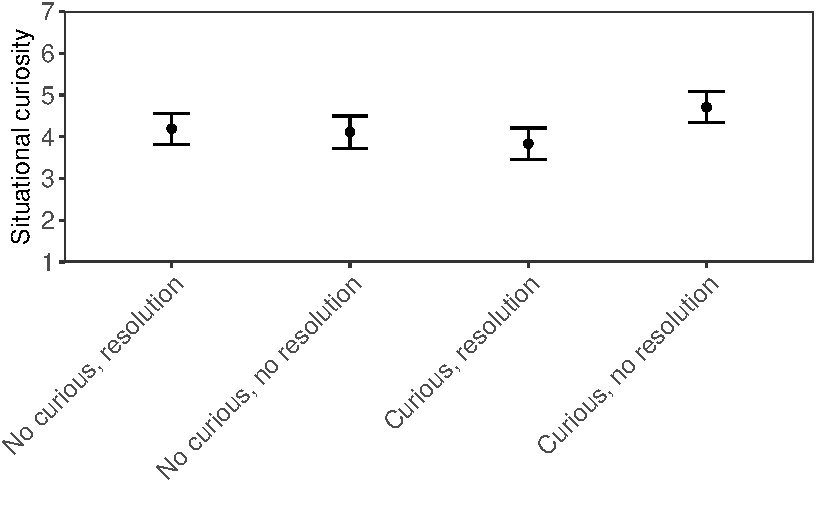
\includegraphics[keepaspectratio]{curiosity_student-pilot_data-analysis_files/figure-pdf/fig-asitcur-1.pdf}}

}

\caption{\label{fig-asitcur}Mean of situational curiosity by
experimental condition for the astronomy issue.}

\end{figure}%

\begin{figure}

\centering{

\pandocbounded{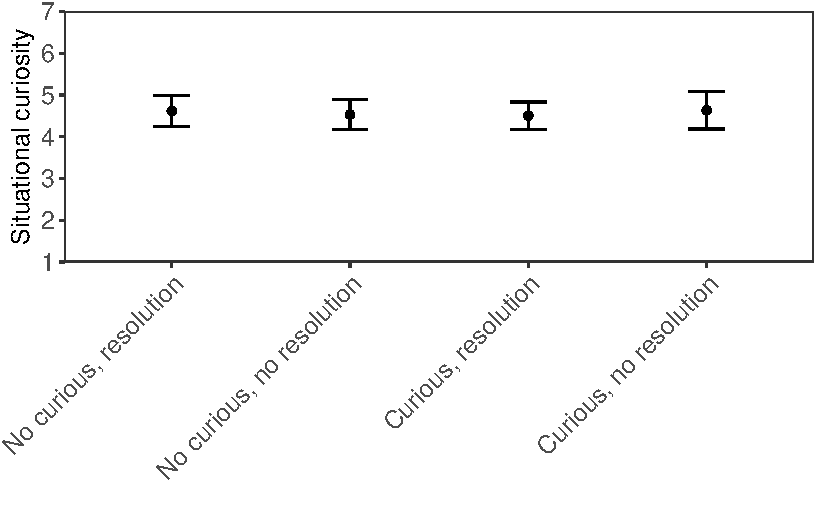
\includegraphics[keepaspectratio]{curiosity_student-pilot_data-analysis_files/figure-pdf/fig-rsitcur-1.pdf}}

}

\caption{\label{fig-rsitcur}Mean of situational curiosity by
experimental condition for the rain/geosmin issue.}

\end{figure}%

\section{Information Seeking}\label{information-seeking}

\begin{figure}

\centering{

\pandocbounded{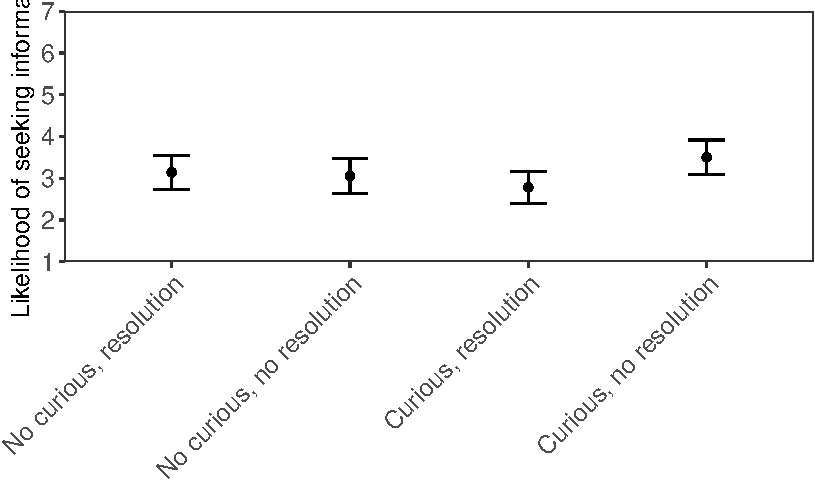
\includegraphics[keepaspectratio]{curiosity_student-pilot_data-analysis_files/figure-pdf/fig-ainfoseek-1.pdf}}

}

\caption{\label{fig-ainfoseek}Mean of information seeking by
experimental condition for the astronomy issue.}

\end{figure}%

\begin{figure}

\centering{

\pandocbounded{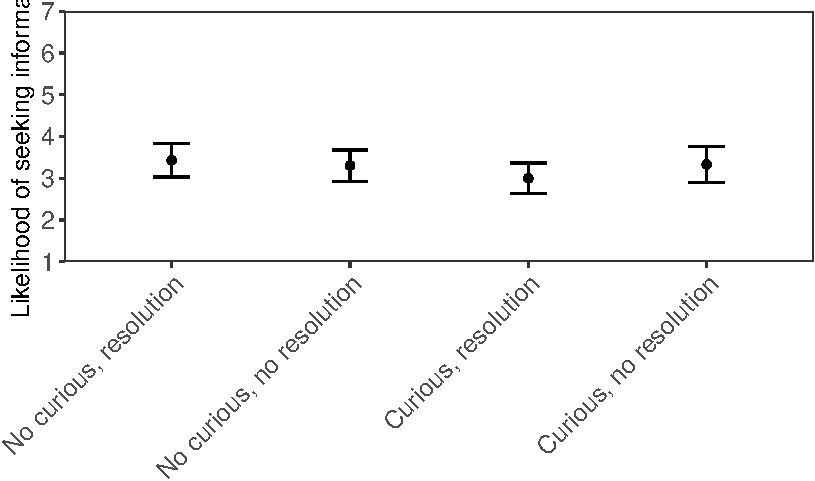
\includegraphics[keepaspectratio]{curiosity_student-pilot_data-analysis_files/figure-pdf/fig-rinfoseek-1.pdf}}

}

\caption{\label{fig-rinfoseek}Mean of information seeking by
experimental condition for the rain/geosmin issue.}

\end{figure}%

\section{Provided Closure}\label{provided-closure}

\begin{figure}

\centering{

\pandocbounded{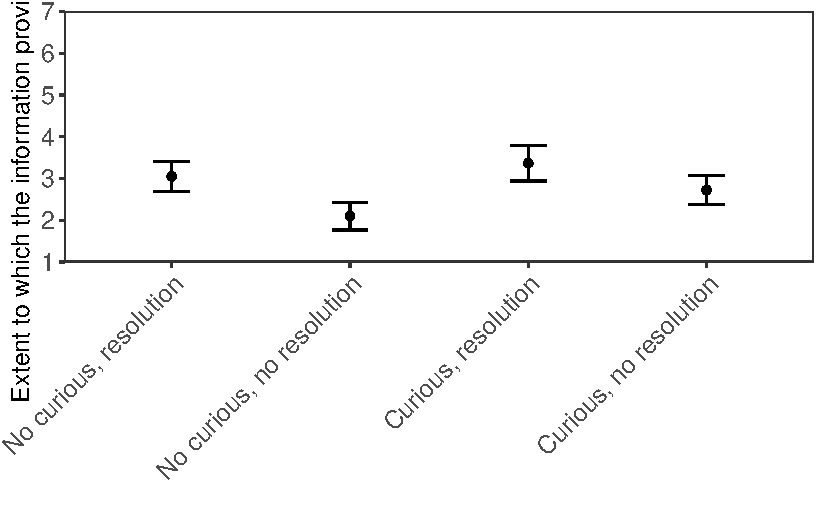
\includegraphics[keepaspectratio]{curiosity_student-pilot_data-analysis_files/figure-pdf/fig-aclosure-1.pdf}}

}

\caption{\label{fig-aclosure}Mean of index tapping the extent to which
the information provided closure by experimental condition for the
astronomy issue.}

\end{figure}%

\begin{figure}

\centering{

\pandocbounded{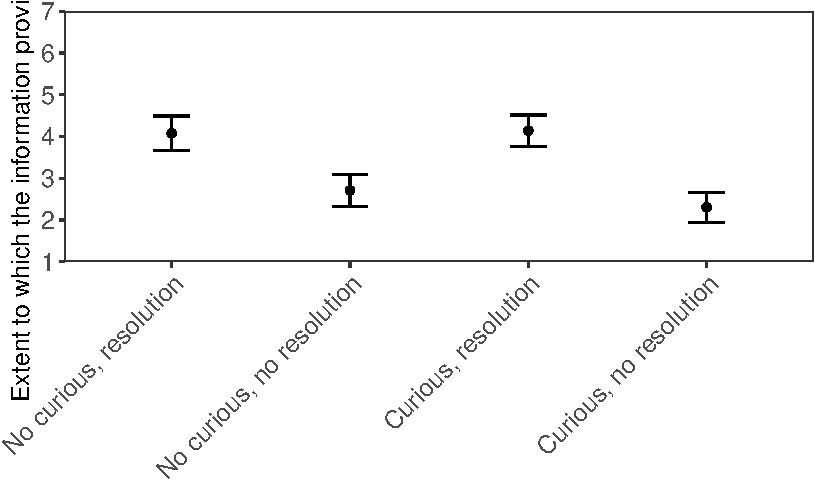
\includegraphics[keepaspectratio]{curiosity_student-pilot_data-analysis_files/figure-pdf/fig-rclosure-1.pdf}}

}

\caption{\label{fig-rclosure}Mean of index tapping the extent to which
the information provided closure by experimental condition for the
rain/geosmin issue.}

\end{figure}%




\end{document}
